% SPDX-License-Identifier: CC-BY-SA-4.0
% Author: Matthieu Perrin
% Part: 
% Section: 
% Sub-section: 
% Frame: 

\begingroup

\begin{frame}{Génération d'un automate}
  \SetKwData{Input}{motif}

  \vspace{-2cm}
  Soit $\Sigma$ un alphabet.

  \begin{minipage}{8cm}
    \begin{block}{Théorème}
      Tout langage rationnel
      est reconnaissable par un automate fini non-déterministe
      $$ \alert{\textsc{rat}_\Sigma \subseteq  \textsc{rec}_\Sigma} $$
    \end{block}
  \end{minipage}
  \begin{block}{Démonstration}
    Algorithme de Thompson
    \begin{description}
    \item [Entrée :] expression rationnelle \structure{$\Input \in \textsc{rat}_\Sigma$}
    \item [Sortie :] automate fini non-déterministe \structure{$A$} tel que $\mathcal{L}(A) = \mathcal{S}(\Input)$ 
      \begin{itemize}
      \item par récurrence sur la structure de $\Input$
      \item construit des automates \alert{normalisés}
      \end{itemize}
    \end{description}
  \end{block}

  \vspace{-6.7cm}\hspace\fill
  \begin{minipage}{2.5cm}
    \centering
    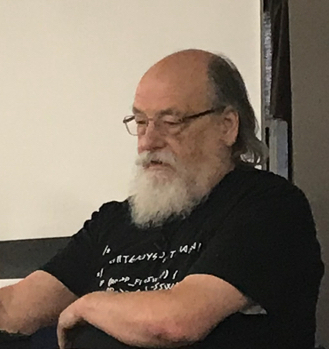
\includegraphics[width=2.5cm]{img/Thompson}
    
    Ken Thompson\footnote[frame,1]{Prix Turing 1983 avec Dennis Ritchie pour le développement d'Unix}
  \end{minipage}\hspace{5mm}
\end{frame}
\endgroup
